\chapter{Θεωρητικό Υπόβαθρο}
\label{chap:background}

\section{Cloud computing}
Εδώ και αρκετό καιρό γίνεται συχνά ανφορά στο "Cloud", αλλά και σε αυτή την
εργασία έχει αναφερθεί αρκετές φορές ο όρος "cloud computing". Παρά τη δημοφιλία
του όρου, δεν υπάρχει ακριβής ορισμός. Εντούτοις, θα χρησιμοποιηθεί ο ορισμός
που έχει δωθεί από το NIST (National Institute of Standards and Technology of
USA) ~\cite{mell2011nist}. Το cloud computing (υπολογιστικό νέφος με ελληνικούς
όρους) είναι η κατ' αίτηση διαδικτυακή κεντρική διάθεση υπολογιστικών πόρων
(όπως δίκτυο, εξυπηρετητές, εφαρμογές και υπηρεσίες) με υψηλή ευελιξία, ελάχιστη
προσπάθεια από τον χρήστη και υψηλή αυτοματοποίηση. Ωστόσο, είναι συχνό
φαινόμενο να αναφερόμαστε με το συγκεκριμένο όρο τόσο στις υπηρεσίες που είναι
διαθέσιμες μέσω διαδικτύου με τη μορφή μίας υπηρεσίας ιστού όσο και στο υλικό
και λογισμικό που απαρτίζουν την υποδομή που προσφέρει αυτές τις υπηρεσίες. 

\subsection{Χαρακτηριστικά του cloud computing}

Πέρα από τον ορισμό το NIST~\cite{mell2011nist}, περιγράφει και τα ακόλουθα
βασικά χαρακτηριστικά του cloud computing: 

\begin{itemize}
\item παροχή υπηρεσίας κατ’ απαίτηση: Οι χρήστες έχουν τη δυνατότητα να
τροποποιήσουν τους πόρους που προσφέρονται, χωρίς την ανθρώπινη διαμεσολάβηση
από την πλευρά του παρόχου του cloud. 
\item ευρυζωνική δικτυακή πρόσβαση: Οι υπηρεσίες είναι διαθέσιμες από το
διαδίκτυο.
\item Διάθεση πόρων σε περισσότερους χρήστες: Οι πόροι μπορούν να διατεθούν
ανάμεσα σε πολλούς χρήστες χωρίς να δημιουργούνται προβλήματα.
\item ταχεία ελαστικότητα/επεκτασιμότητα: Οι πόροι μπορούν να ανακατεμηθούν,
είτε αυτόματα είτε κατ' απαίτηση, χωρίς περιορισμούς και χωρίς να επηρεάζεται η
ομαλή λειτουργία άλλων υπηρεσιών.
\item μετρήσιμη υπηρεσία: Η χρήση των πόρων καταγράφεται και παρουσιάζεται τόσο
στον πάροχο όσο και στον πελάτη.
\end{itemize}

\subsection{Μοντέλα υπηρεσιών}

Σύμφωνα με το NIST~\cite{mell2011nist}, τα μοντέλα υπηρεσιών του cloud είναι τα
εξής:

\vspace{2ex}
\underline{Λογισμικό ως Υπηρεσία (SaaS)}

\vspace{1ex}
Η υπηρεσία που παρέχεται στο χρήστη είναι αυτή μία εφαρμογής που τρέχει  στην
υποδομή του παρόχου. Ο χρήστης δε χρειάζεται να γνωρίζει τίποτα σχετικά με την
υποδομή που υποστηρίζει την εφαρμογή, ούτε έχει τη δυνατότητα να τροποποιήσει
πολλά πράγματα πέρα ίσως από κάποιες ρυθμίσεις που προσφέρει η εφαρμογή. Οι
εφαρμογές αυτές είναι προσβάσιμες μέσα από κάποιο λογιμικό πελάτη που προσφέρει
ο πάροχος ή ακόμα και από ένα πειηγητή ιστού (web browser).

\vspace{2ex}
\underline{Πλατφόρμα ως υπηρεσία (PaaS)}

\vspace{1ex}
Σε αυτή την περίπτωση ο χρήστης έχει τη δυνατότητα της δημιουργίας εφαρμογών
ή/και περιβάλλοντων εφαρμογών, χρησιμοποιώντας προγραμματιστικά εργαλεία και
υπηρεσίες που παρέχονται από τον πάροχο. Ο χρήστης δεν μπορεί να ελέγξει και να
διαχειριστεί την υποδομή του cloud, ωστόσο έχει τον έλεγχο των αναπτυγμένων
εφαρμογών και ενδεχομένως των ρυθμίσεων διαμόρφωσης για το περιβάλλον φιλοξενίας
αυτών των εφαρμογών.

\vspace{2ex}
\underline{Υποδομή ως υπηρεσία (IaaS)}

\vspace{1ex}
Οι παροχές προς το χρήστη είναι υπολογιστικοί πόροι όπως επεξεργαστές,
αποθηκευτικός χώρος και δίκτυο στα οποία μπορεί αναπτύξει και να τρέξει
λειτουργικά συστήματα και εφαρμογές. Παρά τη δυνατότητα να τροποποιήσει την
ποσότητα των πόρων, ο χρήστης δεν έχει παραπάνω έλεγχο ως προς την υποδομή του
cloud. 

\begin{figure}[htp]
\centering
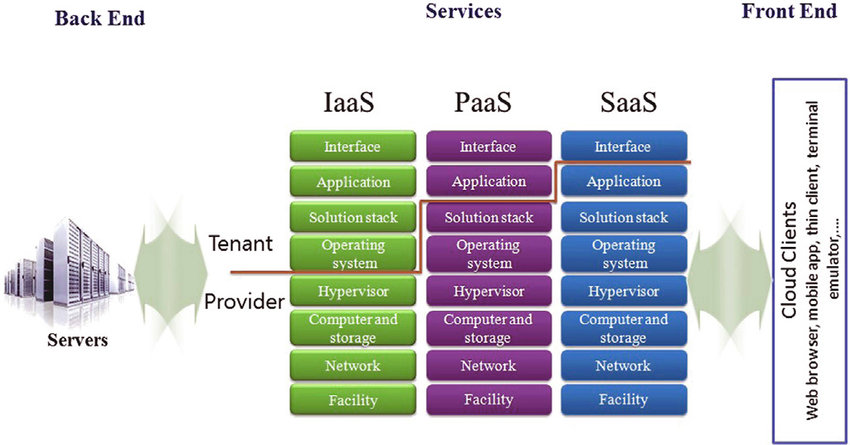
\includegraphics[scale=0.50]{figures/Cloud-service-stack.png}
\caption{Cloud services\label{fig1}}
\end{figure}

\newpage
Όπως βλέπουμε και από το σχήμα ~\ref{fig1}, όσο περισσότερη ευελιξία προσφέρει
ένα μοντέλα τόσο περισσότερο έλεγχο έχει και ο χρήστης στις υπηρεσίες που
λαμβάνει. Για παράδειγμα στην περίπτωση SaaS, ο χρήστης έχει το λιγότερο έλεγχο,
σε αντίθεση με την περίπτωση IaaS όπου ο χρήστης μπορεί πλέον να αποκτήσει
έλεγχο ακόμα και στο λειτυργικό σύστημα.

\section{Εικονικοποίηση}

Στην επιστήμη των υπολογιστών ο όρος εικονικοποίηση (\EN{virtualization}) περιγράφει
ένα μηχανισμό αφαίρεσης, που με τη χρήση "εικονικών υπολογιστικών πόρων", έχει
ως σκοπό την απόκρυψη λεπτομερειών για την υλοποίηση ή την κατάσταση των φυσικών
πόρων. Με το μηχανισμό αυτό ένας φυσικός πόρος μπορεί να παρουσιαστεί ως μία
πλειάδα εικονικών φυσικών πόρων, ή αντίστροφα μία πλειάδα φυσικών πόρων να
παρουσιαστούν ως ένας ενιαίος εικονικός πόρος. Ανάλογα σε ποιο
επίπεδο στη στοίβα του λογισμικού υλοποιείται η εικονικοποίηση, υπάρχουν και τα
αντίστοιχα πλεονεκτήματα, αλλά σε γενικές γραμμές κάποια από τα  πλεονεκτήματα
της εικονικοποίησης είναι:

\begin{itemize}
	\item Καλύτερη αξιοποίηση και διαμοιρασμός των πόρων.
	\item Ασφάλεια μεσω της απομόνωσης των υπηρεσιών.
	\item Δυνατότητα προσομοίωσης περιβαλλόντων που δεν είναι φυσικά
		διαθέσιμα.
	\item Δυνατότητα αποθήκευσης, μεταφοράς και επαναφοράς της κατάστασης
		των υπηρεσιών που προσφέρονται μέσω της εικονικοποίησης.
\end{itemize}

Η εικονικοποίηση μπορεί να υλοποιηθεί σε διάφορα επίπεδα, όπως στο δίκτυο, στον
αποθηκευτικό χώρο, στο hardware, στο λειτουργικό σύστημα κ.α. Η συγκεκριμένη
εργασία ασχολείται κυρίως με την εικονικοποίηση σε επίπεδο υλικού, ωστόσο είναι
συχό φαινόμενο να συγκρίνονται οι unikernels με τα containers. Για το λόγο αυτό
θα γίνει μία σύντομη παρουσίαση της εικονικοποίησης σε επίπεδο λειτουργικού
συστήματος, ενώ μετά από αυτή την περιγραφή, όταν χρησιμοποιείται ο όρος
εικονικοποίηση θα εννοείται εικονικοποίηση επιπέδου υλικού. 

\subsection{Εικονικοποίηση σε επίπεδο λειτουργικού συστήματος}
Η εικονικοποίηση σε επίπεδο λειτουργικού συστήματος είναι νεότερη σε σχέση με
αυτή σε επίπεδο υλικού, ωστόσο έχει καταφέρει να συγκεντρώσει αρκετή προσοχή τα
τελευταία χρόνια. Ο πυρήνας του λειτουργικού συστήματος επιτρέπει την ύπαρξη
παραπάνω από ενα, απομονωμέα userspace instances τα οποία ονομάζονται
containers, virtualization engines ή jails. Όπως φαίνεται στο σχήμα
~\ref{fig2} όλα τα containers μοιράζονται τον
ίδιο πυρήνα πάνω από τον οποίο βρίσκεται το στρώμα που είναι υπεύθυνο για την εικονικοποίηση. 

Το γεγονός ότι τα containers μοιράζονται τον ίδιο πυρήνα κάνει το μέγεθο τους
αρκετά μικρό, αφού δε χρειάζεται να συμπεριλάβουν κάποιο λειτουργικό σύστημα.
Επιπλέον, οι χρόνοι εκκίνησης τους είναι αρκετά μικροί, χωρίς να χρειάζεται να
καταναλωθεί πολύ μνήμη για τη λειτουργεία των containers. Eπιπροσθέτως, τα
containers είναι ανεξάρτητα από το φυσικό μηχάνημα, καθώς η εικονικοποίηση
γίνεται με τη χρήση του κατάλληλου λογισμικού χωρίς να χρειάζεται κάποια
υποστήριξη από το hardware. Τέλος, τα containers επιτρέπουν το εύκολο
πακετάρισμα τόσο των εφαρμογών όσο και των κατάλληλων ρυθμίσεων, που σε
συνδυασμό με την ανεξαρτησία από το hardware, δίνουν τη
δυνατότητα για την εύκολη μεταφορά τους σε διαφορετικά μηχανήματα.

\newpage
\begin{figure}[htp]
\centering
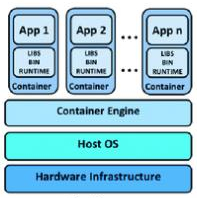
\includegraphics{figures/containers.jpg}
\caption{Εικονικοποίηση σε επίπεδο λειτουργικού συστήματος\label{fig2}}
\end{figure}

Δυστυχώς, όλα αυτά τα πλεονεκτήματα έρχονται με κάποιο κόστος, με το μεγαλύτερο
να είναι αυτό της ασφάλειας. Αν και οι υποστηρικτές των containers θεωρούν ότι
με τις κατάλληλες ρυθμίσεις τα containers μπορούν να γίνουν ασφαλή, δεν
προσφέρουν την ίδια ασφάλεια με την εικονικοποίηση σε επίπεδο
υλικού~\cite{hayden2015securing}. Τα containers δεν έχουν τη δυνατότητα να
προσφέρουν τόσο ισχυρή απομόνωση όσο προσφέρει η εικονικοποίηση σε επίπεδο
υλικού. Τα αποτελέσματα από την παραβίαση της απομόνωσης μπορεί να είναι από την
απόκτηση πληροφοριών σχετικά με το host μηχάνημα ή άλλων containers, μέχρι την
απόκτηση ελέγχου του λειτουργικού συστήματος στον
host~\cite{gao2017containerleaks}. 

Η σύγκριση τψν δύο ειδών εικονικοποίησης είναι ένα ανοιχτό ζήτημα το οποίο
δύσκολα θα λυθεί σύντομα~\cite{eder2016hypervisor}. Άλλωστε και τα δύο είδη,
αναπτύσσονται ταχύτατα, προσφέροντας συνεχώς νέες δυνατότητες και μειώνοντας τα
προβλήματα που υπάρχουν. Σε μία προσπάθεια να ενοποιηθούν τα θετικα των δύο
ειδών, είναι συχνή η χρήση εικονικών μηχανών μέσα στις οποίες τρέχουν
containers. Με αυτό τον τρόπο βελτιώνεται η ασφάλεια σε βάρος όμως της απόδοσης,
καθώς πλέον χρειάζονται πόροι και για την εκτέλεση του απαραίτητου  λογισμικού 
που θα επιτρέψει την υπάρξη εικονικών μηχανών.

\subsection{Εικονικοποίηση σε επίπεδο υλικού}

Η εικονικοποίηση σε επίπεδο υλικού, ή απλά εικονικοποίηση για το υπόλοιπο της
συγκεκριμένης εργασίας, επιτρέπει τη λειτουργία ενός ολόκληρου υπολογιστικού
συστήματος μέσα από έναν άλλον. Τα εμφωλευμένα υπολογιστικά συστήματα
αναφέρονται ως guests, ενώ το υπολογιστικό σύστημα στο οποίο πραγματοποιείται η
εικονικοποίηση αναφέρεται ως host. Ένας guest εκτελείται μέσα σε μία εικονική
μηχανή (virtual machine - VM), την οποία οι Popek και Goldberg
~\cite{popek1974formal} ορίζουν ως εξής: “ένα αποδοτικό και απομονωμένο
αντίγραφο μιας πραγματικής μηχανής”. Κάθε εικονική μηχανή είναι ανεξάρτητη τόσο
από το host, όσο και άπο άλλες τυχόν εικονικές μηχανές που μπορεί να υπάρχουν.
Με αυτού του είδους την εικονικοποίηση, κάθε εικονική μηχανή έχει την
ψαυδαίσθηση ότι κατέχει αποκλειστικά τους πόρους που της έχουν διατεθεί.

Απαραίτητο συστατικό για να επιτευχθούν όλα τα παραπάνω είναι ο επόπτης
(hypervisor). Ο επόπτης, σύμφωνα με τους Popek και Goldberg έχει τρία
συγκεκριμένα χαρακτηριστικά ~\cite{popek1974formal}:
\begin{enumerate}
	\item o επόπτης παρέχει ένα περιβάλλον όμοιο με το πραγματικό 
			υπολογιστικό σύστημα,
	\item τα προγράμματα που τρέχουν στο περιβάλλον που δημιουργείται θα
		πρέπει να έχουν στη χειρότερη περίπτωση μικρές μειώσεις στην
		ταχύτητα εκτέλεσης,
	\item o επόπτης έχει πλήρη έλεγχο των πόρων.
\end{enumerate}

Ο ρόλος του επόπτη μοιάζει με το ρόλο του λειτουργικού συστήματος, 
με τις εικονικές μηχανές να έχουν το ρόλο των διεργασιών. Ο επόπτης
χρονοδρομολογεί τις εικονικές μηχανές στη CPU, μοιράζει γενικότερα τους
διαθέσιμους πόρους στα εικονικά μηχανήματα, εκτελεί εκ μέρους των εικονικών
μηχανών "προνομιούχες εντολές" και είναι αυτός που διαχειρίζεται τις εικονικές
μηχανές (δημιουργία, εκκίνηση, τερματισμός κ.λ.π).

Όπως βλέπουμε στο σχήμα ~\ref{fig3} υπάρχουν δύο διαφορετικά είδη εποπτών,
ανάλογα με το που βρίσκονται στο σύστημα. 
\begin{itemize}
	\item \textbf{Type 1 - Bare metal/native} \\
		Σε αυτή την περίπτωση ο επόπτης εκτελείται πάνω από το υλικό του
		συστήματος, χωρίς να παρεμβάλλεται κάποιο λειτουργικό σύστημα.
		Είναι υπεύθυνος για τη χρονοδρομολόγηση των εικονικών μηχανών,
		τη διαχείριση της μνήμης και των πόρων καθώς και άλλων
		λειτουργιών. Χρησιμοποιεί δικούς του drivers για τη διαχείριση
		του υλικού και για την εξυπηρέτηση των I/O λειτουργιών των
		guest. 
	\item \textbf{Type 2 - Hosted} \\
		Σε αυτή την περίπτωση ο επόπτης εκτελείται πάνω από ένα
		λειτουργικό σύστημα, σαν ένα συνηθισμένο πρόγραμμα στο
		\EN{user space.} Αποτελούν ένα ενδιάμεσο στρώμα μεταξύ του host και
		του guest, δημιουργώντας το κατάλληλο περιβάλλον για τις
		εικονικές μηχανές. Δε χρειάζονται ειδικοί drivers για 
		το υλικό, καθώς αυτοί παρέχονται από το λειτουργικό σύστημα του
		host. Από την άλλη, οι I/O λειτουργίες και διάφορες άλλες
		"προνομιούχες εντολές" του guest θα πρέπει να
		περάσουν μέσα από τον hypervisor και μετά να εξυπηρετηθούν από
		τον host, δημιοργώντας επιπλέον κόστος στην εκτέλεση τους. 
\end{itemize}

\begin{figure}[htp]
\centering
	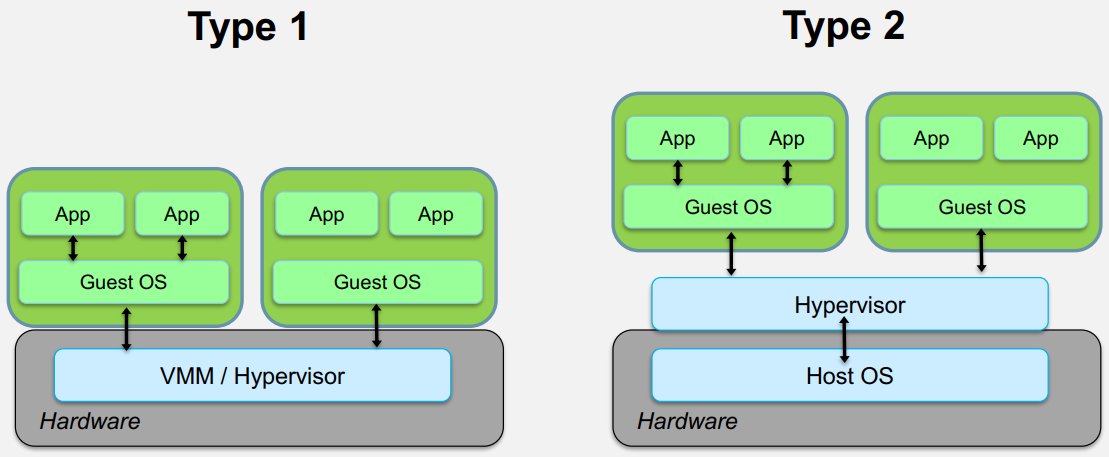
\includegraphics[scale=0.3]{figures/zcBClDR.png}
\caption{Εικονικοποίηση σε επίπεδο υλικού\label{fig3}}
\end{figure}

Εκτός από το διαχωρισμό των εποπτών, γίνεται και διαχωρισμός και στις τεχνικές
που χρησιμοποιούνται για να επιτευχθεί η εικονικοποίηση. Οι τεχνικές αυτές
βασίζονται τόσο στη δυνατότητα που προσφέρει ειδικό υλικό για την υποστήριξη της
εικονικοποίησης, όσο και στο βαθμό συνεργασίας μεταξύ του επόπτη με το εικονικό
μηχάνημα. Θα αναφερθούμε σε τρεις από αυτές τις τεχνικές, την πλήρη
εικονικοποίηση (full virtualization), την παραεικονικοποίηση
(paravirtualization) και τέλος την εικονικοποίηση υποστηριζόμενη από το υλικό
(hardware-assisted virtualization). 

\vspace{2ex}
\underline{Full virtualization}

\vspace{1ex}

Στην πλήρη εικονικοποίηση ο guest δεν έχει υποστεί καμία αλλαγή και εκτελείται
όπως και στην περίπτωση που εκτελείται απευθείας σε ένα φυσικό υπολογιστικό
σύστημα. Απο τη μεριά του ελεγκτή, θα πρέπει να γίνει πλήρης προσομοίωση του
υλικού ώστε να δίνει την ψευδαίσθηση στον guest ότι επικοινωνεί απευθείας με το
υλικό. Ωστόσο δημιουργείται ένα πρόβλημα, το λειτουργικό σύστημα του guest
εκτελείται σε unprivileged mode, οπότε δεν μπορεί να εκτελέσει προνομιούχες
εντολές. Η λύση σε αυτό το πρόβλημα είναι η τεχνική trap-and-emulate
~\cite{adams2006comparison}, κατά την οποία όταν ο guest προσπαθεί να εκτελέσει
μία προνομιούχα εντολή, δημιουργείται μία εξαίρεση (trap) στον hypervisor, καθώς
ο guest βρίσκεται σε unprivileged mode. Ύστερα, ο hypervisor παίρνει τον έλεγχο
και προσομοιώνει ή εκτελεί την προνομοιούχα εντολή για λογαριασμό του guest. 

H συγκεκριμένη λύση δεν είναι αρκετή για όλες τις αρχιτεκτονικές. Μία από αυτές
τις αρχιτεκτονικές είναι και η x86. Στην x86 αρχιτεκτονική ορισμένες εντολές
δεν προκαλούν trap όταν εκτελούνται σε unprivileged mode, παρά το γεγονός ότι
για την εκτέλεση τους είναι ανάγκη να βρίσκονται σε privileged mode
(non-virtualizable instructions). Μία από
αυτές τις εντολές είναι η popf, η οποία ενώ αλλάζει τόσο τα ALU flags όσο και τα
flags του επεξεργαστή δεν προκαλεί κάποιο trap με αποτέλεσμα να αγνοούνται οι
αλλαγές στα flags του επεξεργαστή. Για την αντιμετόπιση του συγκεκριμένου
προβλήματος χρησιμοποείται από τους επόπτες η τεχνική του binary translation
~\cite{adams2006comparison}. 
Όταν ο guest βρίσκεται σε unprivileged mode όλες οι εντολές εκτελούνται
κανονικά, ενώ όταν μεταβεί στον πυρήνα και σε privileged mode τότε ο hypervisor
μεταφράζει τις εντολές που δεν προκαλούν trap σε ένα νέο σύνολο εντολών που θα
επιφέρουν τις επιθυμητές αλλαγές στην εικονική μηχανή. 

Μπορούμε να παρατηρήσουμε εύκολα ότι και στις δύο περιπτώσεις η απόδοση θα
μειωθεί σημαντικά, λόγω της ανάμειξης του \EN{hypervisor}. Ιδιαίτερα στην περίπτωση
του binary translation το κόστος της παρακολούθησης και μετάφρασης των εντολών
του guest είναι αρκετά μεγάλο. 

\vspace{2ex}
\underline{Paravirtualization}

\vspace{1ex}

Στην παραεικονικοποίηση ο guest γνωρίζει ότι δεν εκτελείται απευθείας στο υλικό
και "συνεργάζεται" κατάλληλα με τον hypervisor. Απαιτείται λοιπόν, η τροποποίηση
του guest, ώστε να αντικατασταθούν οι non-virtualizable εντολές, με κατάλληλες
εντολές (hypercalls) που δίνουν τον έλεγχο στο hypervisor και αυτός με τη σειρά του διεκπαιρεώνει την αντίστοιχη λειτουργία. Επιπλέον ο hypervisor μπορεί να
υποστηρίξει και κάποιες άλλες εντολές, που χρησιμοποιούνται για άλλες σημαντικές
λειτουργίες του πυρήνα, όπως διαχείρηση μνήμης, διαχείριση διακοπών κ.α. 

Με αυτό τον τρόπο μειώνεται σημαντικά το κόστος της εικονικοποίησης, αφού ο
guest γνωρίζει ότι εκτελείται σε εικονικό περιβάλλον και μπορεί να
βελτιστοποιηθεί για τις συγκεκριμένες συνθήκες. Παράλληλα γίνεται
δυνατόν να εικονικοποιηθούν αρχιτεκτονικές όπως η x86 χωρίς σημαντική μείωση
της απόδοσης αποφεύγοντας το binary translation. Από την άλλη, o guest
τροποποιείται αρκετά για να μπορέσει να "συνεργαστεί" με τον επόπτη. Συνεπώς, 
μειώνεται η δυνατότητα μεταφοράς του σε διαφορετικά συστήματα (π.χ. διαφορετικό
επόπτη), ενώ ταυτόχρονα αυξάνει το κόστος συντήρησης του καθώς οποιεσδήποτε
αλλάγές ή αναβαθμίσεις στον πυρήνα του guest θα πρέπει να τροποποιηθούν
κατάλληλα για την υποστήριξη της παραεικονικοποίησης.

\vspace{2ex}
\underline{Hardware-assisted virtualization}

\vspace{1ex}

Η συγκεκριμένη μέθοδος ουσιαστικά έχει τα ίδια χαρακτηριστικά με τη μέθοδο της
πλήρης εικονικοποίησης. Ο guest δε χρειάζεται να υποστεί καμία αλλαγή, ενώ
εισάγεται κατάλληλο hardware το οποίο διευκολύνει την εικονικοποίηση. Πρόκειται
για επεκτάσεις των επεξεργαστών με στόχο την αύξηση της απόδοσης και της
ασφάλειας της εικονικοποίησης. Αυτές οι επεκτάσεις είναι γνωστές ως επεκτάσεις
εικονικοποίησης (virtualization extensions). 

Ένα από τα βασικά στοιχεία αυτών των επεκτάσεων είναι η δημιουργία ενός νέου
επιπέδου εκτέλεσης, αυτό του guest στο οποίο μπορούν να εκτελεστούν τόσο
privileged όσο και unprivileged εντολές. Συνεπώς, δε χρειάζεται πλέον να
γίνονται trap οι privileged εντολές του guest, αλλά αυτές μπορούν να εκτελεστούν
απευθείας, χωρίς μάλιστα να επηρεάζεται ο host από την εκτέλεση τους. Οι
επεκτάσεις αφορούν ακόμα τη διαχείριση μνήμης, αλλά και των διακοπών. Πλέον η
εκτέλεση του guest συνεχίζεται αδιάκοπα μέχρι την ικανοποίηση κάποιας συνθήκης,
όπως για παράδειγμα ένα page fault, όπου τότε ο έλεγχος μεταφέρεται στον host
(VM exit). 

Με αυτό τον τρόπο επιτυγχάνεται υψηλή απόδοση για την εικονικοποίηση χωρίς να
είναι απαραίτητες οι αλλαγές στον guest. O πιο σημαντικός παράγοντας απόδοσης
για την εν λόγω τεχνική είναι το πλήθος των VM exits, καθώς πρόκειται για μία
χρονοβόρα διαδικασία ~\cite{agesen2012software}. Μάλιστα πολλές από αυτές τις
επεκτάσεις έχουν δημιοργηθεί για  ακριβώς αυτό το σκοπό, δηλαδή τη μείωση των VM
exits. 


\subsection{QEMU/KVM}

Το Qemu ~\cite{bellard2005qemu} είναι ένας επόπτης τύπου 2 και πρόκειται για
έναν από τους πιο γνωστούς επόπτες. Με την τεχνική του full virtualization και
συγκεκριμένα με τη μέθοδο του dynamic binary translation, υποστηρίζει τη
φιλοξενεία πολλών λειτουργικών συστημάτων χωρίς να απαιτείται κάποια αλλαγή σε
αυτά. Πέρα από τη λειτουργία του επόπτη, μπορεί να λειτουργήσει και ως
προσομοιωτής υλικού. Το Qemu έχει τη δυνατότητα να προσομοιώσει διαφορετικές
αρχιτεκτονικές από αυτή που διαθέτει ο host, πληθώρα από κάρτες δικτύου,
σκληρούς δίσκους, περιφερειακές συσκευές κ.λ.π.. Mε αυτό τον τρόπο μπορεί να
χρησιμοποιηθεί και για εφαρμογές που έχουν υλοποιηθεί για διαφορετική
αρχιτεκτονική να εκτελεστούν στην αρχιτεκτονική που διαθέτει ο host. 

Οι εικονικές μηχανές που εκτελούνται στον ίδιο host, συχνά επικοινωνούν μεταξύ
τους. Συνήθως πρόκειται για πλήρη υπολογιστικά συστήματα, συνεπώς για την
επικοινωνία μεταξύ τους θα μπορούσε να χρησιμοποιηθεί ό,τι χρησιμοποιειταί
μεταξύ φυσικών υπολογιστικών συστημάτων (π.χ. TCP/IP sockets). Μάλιστα ειδικά
στη συγκεκριμένη περίπτωση οι επόπτες μπορούν να αντιληφθούν ότι πρόκειται για
επικοινωνία μεταξύ εικονικών μηχανών που ελέγχουν οπότε και χρησιμοποιούν
διάφορες βελτιστοποιήσεις, προκειμένου να μη χρειαστεί να περάσουν τα πακέτα
πέρα από το host. Εντούτοις, συχνά πολλές εικονικές μηχανές δε χρειάζονται
δίκτυο και δημιουργείται η ανάγκη για επικοινωνία μεταξύ τους 
ή ακόμα και με το host. Επιπλεόν πολλές φορές είναι χρήσιμο εικονικές μηχανές
να μοιράζονται μνήμη μεταξύ τους. Έτσι έχουν δημιουργηθεί αρκετές μέθοδοι για
τον διαμοιρασμό μνήμης και ενδοεπικοινωνίας μεταξύ εικονικών μηχανών, αλλά και
μεταξύ του host και των εικονικών μηχανών ~\cite{ren2016shared}. 

Ένας από αυτούς τους μηχανισμούς είναι ο nahanni ή ivshmem (inter-VM shared
memory) ~\cite{macdonell2011shared}. To ivshmem είναι ένας μηχανισμός για το
διαμοιρασμό μνήμης του host με τις εικονικές μηχανές που εκτελούνται στο host.
Μπορεί να χρησιμοποιηθεί τόσο για διαμοιρασμό μνήμης μεταξύ host και guest, όσο
και μεταξύ των guests. To Qemu επιτρέπει τη χρήση αυτού τού μηχανισμού μέσω
μίας PCI συσκευής την οποία πρέπει να υποστηρίξουν οι guests για να
χρησιμοποιήσουν τη συγκεκριμένη περιοχή μνήμης. 

Πολλές φορές το Qemu χρησιμοποιείται από άλλους επόπτες για την εξομοίωση του
υλικού, όπως για παράδειγμα γίνεται από το Xen. Επιπροσθέτως συχνά
χρησιμοποιείται σε συνδυασμό με το kvm (στην περίπτωση υποστήριξης
hardware-assisted virtualization), πετυχαίνοντας υψηλή απόδοση. Το kvm είναι ένα
kernel module του Linux, που μετατρέπει τον πυρήνα σε εναν επόπτη.Ωστόσο, από
μόνο του το kvm δε λειτουργεί ως επόπτης, αλλά ανοίγει μία διεπαφή (/dev/kvm)
μέσω της οποίας μπορούν να χρησιμοποιηθούν οι διάφορες λειτουργίες που
προσφέρει. Σε αυτό τον συνδυασμό (Qemu/Kvm) κάθε εικονική μηχανή εκτελείται ως
μία διεργασία. 

\section{Λειτουργικά συστήματα}

Το λειτουργικό σύστημα είναι ένα πρόγραμμα το οποίο εκτελείται σε ένα
υπολογιστικό σύστημα. Η ειδοποιός διαφορά του με οποιοδήποτε άλλο πρόγραμμα
είναι ότι το πρώτο υπάρχει για να εξυπηρετεί το δεύτερο. Το λειτουργικό σύστημα
διαχειρίζεται το υλικό του υπολογιστικού συστήματος και παρέχει στους
πργαμματιστές των εφαρμογών ένα σαφές αφηρημένο σύνολο πόρων, αντί για το
μπερδεμένο σύνολο που υπάρχει στο υπολογιστικό σύστημα. Χωρίς αυτό, ο
προγραμματιστής μίας οποιασδήποτε εφαρμογής θα έπρεπε να γράψει και τον κατάλλο
κώδικα για το υλικό που χρησιμοποιεί η συγκεκριμένη εφαρμογή (π.χ. αποθήκευση σε
σκληρό δίσκο). Ως εκ τούτου θα σπαταλούσε αρκετό χρόνο σε μη βασικές λειτουργίες
του προγράμματος. Επιπροσθέτως πολλές από αυτές τις λειτουργίες που αφορούν το
υλικό μπορεί να έχουν ήδη υλοποιηθεί από άλλα προγράμματα, σπαταλώντας έτσι
χρόνο για ήδη υπάρχουσες λειτουργίες. 

Η πληθώρα και οι σημαντικές διαφορές στο σκοπό και στις δυνατότητες των
υπολογιστικών συστημάτων οδήγησε στη δημιουργία διαφορετικών ειδών λειτουργικών
συστημάτων. Για παράδειγμα, ένα λειτουργικό σύστημα που έχει δημιουργηθεί με
σκοπό την εκτέλεση του σε προσωπικούς υπολογιστές διαφέρει αρκετά από ένα
λειτουργικό σύσστημα που χρησιμοποιείται σε ενσωματωμένα συστήματα. Το πιο
γνωστό είδος λειτουργικών συστημάτων είναι αυτά του γενικού σκοπού, τα οποία
έχουν ως στόχο να μπορούν να εκτελεστούν σε διάφορα υπολογιστικά συστήματα
προσφέροντας όσο το δυνατόν περισσότερες λειτουργίες. 

Ένας διαφορετικός τρόπος κατηγοριοποίησης των λειτουργικών συστημάτων γίνεται με
τη δομή τους. Αναφέρουμε τις κυριότερες από αυτές τις δομές, οι οποίες είναι τα
μονολιθικά συστήματα, τα πολυεπίπεδα συστήματα και οι μικροπυρήνες.

\begin{itemize}
	\item μονολιθικά συστήματα: η πιο διαδεδομένη οργάνωση, στην οποία
		ολόκληρο το λειτουργικό συστημα εκτελείται ως ένα
		μοναδικό πρόγραμμα σε κατάσταση πυρήνα. Ουσιαστικά πρόκειται για
		ένα μεγάλο εκτελέσιμο δυαδικό πρόγραμμα. Κάθε διαδικασία του
		συστήματος μπορεί να καλέσει οποιαδήποτε άλλη. 
	\item πολυεπίπεδα συστήματα: το λειτουργικό σύστημα οργανώνενται σε μία
		ιεραρχία επιπέδων, όπου το καθένα δομείται πάνω στο αμέσως
		κατώτερο του. Κάθε επίπεδο αναλαμβάνει μία διαφορετική
		λειτουργία και μπορεί να χρησιμοποιήσει μόνο λειτουργίες που
		υποστηρίζουν κατώτερα επίπεδα.
	\item μικροπυρήνες: το λειτουργικό σύστημα διαιρείται σε μικρές καλά
		ορισμένες υπομονάδες, από τις οποίες μόνο μία, ο μικροπυρήνας,
		εκτελείται σε κατάσταση πυρήνα ενώ οι υπόλοιπες εκτελούνται σε
		σχετικά λιγότερο ισχυρές κοινές διεργασίες χρήστη.
\end{itemize}

Σε ένα μονολιθικό λειτουργικό συτημα διακρίνονται δύο ξεχωριστά επίπεδα
εκτέλεσης κώδικα. Κάθε επίπεδο έχει διαφορετικούς χώρους μνήμης και διαφορετικά
δικαιώματα πρόσβασης στο υλικό. Τα δύο αυτά επίπεδα είναι ο χώρος χρήστη
(user space), στο οποίο εκτελούνται οι διεργασίες του χρήστη και ο χώρος πυρήνα
(kernel space), στο οποίο εκτελείται ο κώδικας του πυρήνα. Προκειμένου μία
διεργασία να εκτελέσει μία λειτουργία για την οποία δε διαθέτει τα ανάλογα
δικαιώματα, υπάρχει ένας μηχανισμός μέσω του οποίου η διεργασία ζητά από τον
πυρήνα να εκτελέσει τη συγκεκριμένη λειτουργία για λογαριασμό της. Ο μηχανισμός
αυτός ονομάζεται κλήση συτήματος (system call). 

%%Όπως έχει ήδη αναφερθεί ένα λειτουργικό σύστημα διαχειρίζεται το υλικό του
%%υπολογιστικού συστήματος στο οποίο εκτελείται. Οι λεπτομέρειες του ελέγχου και
%%προγραμματισμού μίας συσκευής περικλείονται μέσα σε τμήματα κώδικα που
%%ονομάζεται οδηγός συσκευής και έχει συγκεκριμένο τρόπο επικοινωνίας με τον
%%υπόλοιπο πυρήνα. 

Ένα από τα πρώτα και πιο ιστορικά λειτουργικά συστήματα είναι το UNIX. Το UNIX
επιλέχτηκε ως η βάση για μία τυποποιημένη διεπαφή συστήματος, ωστόσο υπήρχαν και
δημιουργήθηκαν πολλές παραλλαγές του. Συνεπώς, δημιουργήθηκε η ανάγκη για τη
δημιουργία ενός κοινού standard, ώστε να διατηρείται η συμβατότητα μεταξύ αυτών
των διάφορων εκδόσεων του UNIX. Το standard που δημιουργήθηκε ήταν το POSIX, το
οποίο ορίζει μία ελάχιστη διασύνδεση κλήσεων συστήματος που πρέπει να
υποστηρίζουν τα συμβατά συστήματα UNIX. Μάλιστα το POSIX χρησιμοποιείται ακόμα
και στις μέρες μας, ενώ έχουν δημιουργηθεί και κάποιες παραλλαγές του. Το UNIX
επηρέασε σε μεγάλο βαθμό και κάποια από τα πιο δημοφιλη σύγχρονα λειοτυργικά
συστήματα όπως το Linux και αυτά της οικονγένειας BSD. Ένα από αυτά τα
λειτουργικά συστήματα είναι και το NetBSD, το οποίο είναι ένα γενικού σκοπού
λειτουργικό σύστημα. Χρησιμοποιείται συνήθως σε servers και λιγότερο σε
προσωπικούς υπολογιστές, ενώ υποστηρίζει αρκετές αριτεκτονικές. 

%%TODO: isws prepei na grpsw kai gia compilers/cross-compiling

